\section{Literature Review}
\subsection{Force Balances}
\paragraph{}For wind tunnel applications, the wind axes is used as the reference frame. Where, X axis points to the accelerated air; Z axis points downward and; Y axis points to the right in the direction of the wind. In the reference frame above, lift is in the negative z-direction, drag in the negative x-direction and, side force in the negative y-direction.
\paragraph{}Moment components on the x,y,z axes are rolling moment, pitching moment and yawing moment respectively. A three-component force balance can be considered to measure the lift, drag and pitch (angle of attack).
\paragraph{}Force balances can be external or internal. In external force balances the test section lies outside of the wind tunnel test section, whereas in internal force balances the balance is inside the model itself connecting the model to the support structure.
\paragraph{}Several different types of external force balances are available for wind tunnel use
\cite{morris_force_2010}:
\begin{enumerate}
\item Wire
\item Platform
\item Yoke
\item Pyramidal
\end{enumerate}
\begin{center}
	\begin{figure}[!h]
	\centering
	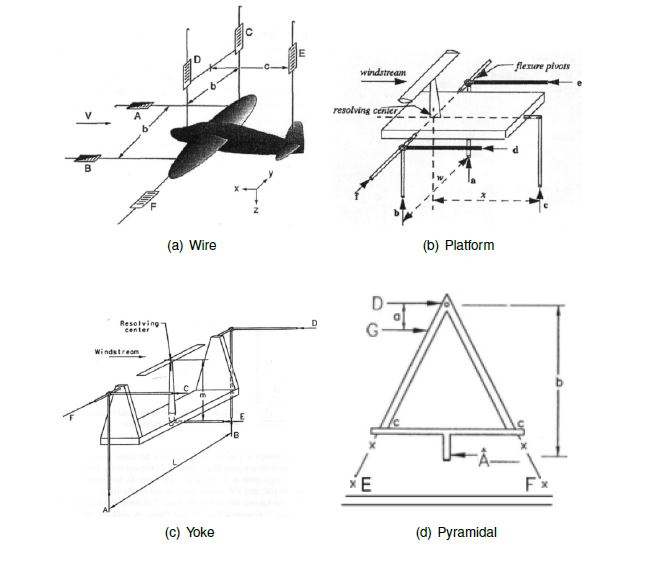
\includegraphics{Figures/Fig6}
	\caption{Typical configurations for external force balances}
	\end{figure}
\end{center}
\paragraph{}In the wire balance, the model under testing is suspended by wires each connected to an extensometer (a sensor that produces an electrical output when submitted to a load and deforms). The shortcoming of the wire balance is the large tare drag caused by the wires which is difficult to quantify. They are also not robust nor versatile enough compared with the other alternatives. 
\paragraph{}The platform balance is relatively easy to construct, assemble and instrument. However, for this balance, forces and torques are coupled and the balance resolving center does not coincide with the center of the tunnel. 
\paragraph{}In the yoke balance configuration, forces and torques are coupled and the balance resolving center coincides with the center of the tunnel. This configuration, however, presents some structural deflections due to the large span of the measuring and support arms.
\paragraph{}The pyramidal balance configuration is a further improvement of the yoke balance in order to overcome the shortcomings of the other balances. It is capable of measuring six components of forces and
torques separately and without coupling,provided that the balance is well assembled and calibrated.

\paragraph{}The different kinds of internal balances can be made based on:
\begin{enumerate}
\item The type of transducer i.e. strain gauge or piezoelectric balance.
\item Shape i.e. box balance and sting balance
\end{enumerate} 
\begin{center}
	\begin{figure}[!h]
	\centering
	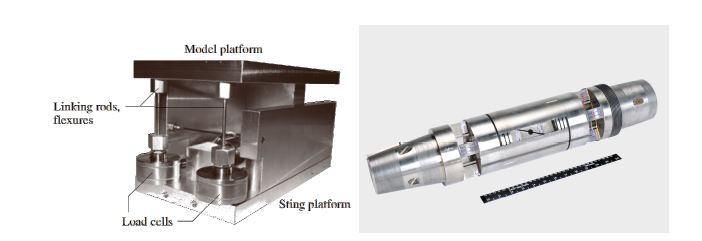
\includegraphics{Figures/Fig7}
	\caption{Typical configurations for internal force balances. \textit{Left to right:} Box balance and sting balance.}
	\end{figure}
\end{center}
\paragraph{}The box balance presents a cubic shape and can either be made of a solid piece of material or from assembled parts. In this configuation, the loads are transferred from the top to the bottom. The sting balance presents a cylindrical shape and the loads are transferred from one end to the other in the longitudinal direction. It can be used to measure forces or torques.
\paragraph{}The advantage of internal force balances is that they minimize the interference caused by the supporting bars in the flow.
\subsection{Sensors}
\subsubsection{Load Sensors}
\paragraph{}Several methods can be used to measure forces and torques in a force balance. These methods can be generally grouped into two:
\begin{enumerate}
\item Hydraulic measuring techniques.
\item Electric measurement techniques.
\end{enumerate}
\paragraph{}Electric measurement techniques are preferred for Force balance applications. One such electric measurement device is the strain gauge. A strain gauge is an electromechanical device whose electrical resistance changes linearly with the strain in the component.
\paragraph{}Metal foil strain gauges are widely used. This type of strain gauge provide more precise strain values than wire strain gauges. However, since the relative changes on electric resistance of the strain gauge are so small, it is necessary to develop an effective method to measure them because each strain gauge would require extremely accurate signal measurements. The solution is to have a set of strain gauges coupled in order to minimize the required accuracy, forming a force transducer i.e. the \textit{Wheatstone bridge}.
	\begin{figure}[!h]
	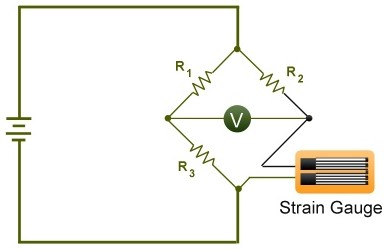
\includegraphics{Figures/Fig9}
	\caption{Wheatstone Bridge Circuit}
	\end{figure}
\paragraph{}Load cells can also be used to measure the drag and lift forces.
\subsubsection{Altitude Sensor}
\paragraph{}It is important to define the desired aerodynamic angles and to guarantee that they are measured accurately in relation to the air stream. One such angle is the angle of attack (\textalpha) shown in Figure 2.4. For this reason, specific devices that provide the attitude measurement should be implemented in order to improve the precision of the results.
\paragraph{}Angle of attack (\textalpha)- angle measured between the longitudinal axis of the model and the direction of the flow on a vertical (Figure 2.4)
\begin{center}
	\begin{figure}[!h]
	\centering
	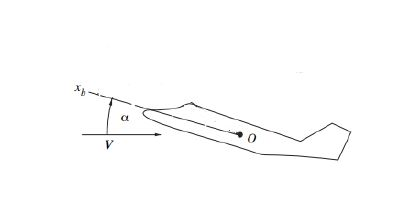
\includegraphics{Figures/Fig10}
	\caption{Angle of attack (\textalpha)}
	\end{figure}
\end{center}